\section{Evaluation}\label{sec:evaluation}
The evaluation focuses on computations that are expected to profit from parallelization, e.g. compute-intensive tasks or tasks over a large set of data. However, using the presented runtime system may also be beneficial for long-running, but not parallelized computations that otherwise would block the main thread and result in a degraded user experience. The evaluation compares the presented work with the alternatives introduced in \cref{sec:related-work} concerning performance and applicability to the following set of problems:

\begin{itemize}
	\item[$\bullet$] Knight Tour: Computes the number of open tours from a given start field. Low memory usage but very high computational needs.
	\item[$\bullet$] Mandelbrot 10'000x10'000: Computation of a Mandelbrot for a given image size. This problem requires a relatively large amount of memory compared to the computational time needed.
	\item[$\bullet$] Risk Profiling: Creates forecasts for the customer's asset development over a period of 15 years under different investment strategies and economic circumstances by using a Monte Carlo simulation. The forecast is used to show the customer how different developments affect planned investments --- e.g. buying a house after ten years. This problem is an instance of a real-world problem~\cite{Kwsoft2016}.
\end{itemize}

The versions used by the evaluated runtime systems are shown in \cref{tab:runtime-system-version}.

\begin{table}
	\centering
	\begin{tabular}{p{0.6\linewidth} l}
		\toprule
		Runtime System & Version \\ \midrule
		Parallel.es & 0.1.14 \\
		Hamsters.js & 3.9.0\footnote{The version used is based on 3.9.0 but contains a fix for input data that is not a typed array (\url{https://github.com/austinksmith/Hamsters.js/issues/16}).} \\
		Parallel.js & 0.2.x\footnote{Latest version from master as mentioned in \cref{sec:related-work}.} \\
		Threads.js & 0.7.2 \\ \bottomrule
	\end{tabular}
	\caption{Versions of Evaluated Runtime Systems}
	\label{tab:runtime-system-version}
\end{table}


\subsection{Applicability}
The applicability is mainly evaluated by comparing the Mandelbrot implementations. The synchronous and Parallel.es based implementations of the Mandelbrot have been introduced in \cref{sec:programming-model} and are shown in \cref{fig:mandelbrot-sync,code:mandelbrot-parallel.es}. The implementation of the per line computation is omitted for brevity since it is almost identical for all libraries. The preliminary focus of the evaluation is on readability and type safety. However, some of the results might be subjective and represent the opinion of the author. The source code for all examples is available on GitHub~\cite{Reiser2016}. 

\paragraph{Parallel.js}
\Cref{fig:mandelbrot-paralleljs} shows the Mandelbrot implementation using the reactive API of Parallel.js. It differs only slightly from the synchronous implementation. A parallel task is created using the \javascriptinline/Parallel/ constructor (line \ref{code:paralleljs-definition}). The first constructor argument is the data to process, the second --- optional ---  is an options object affecting the task execution where the value of the \javascriptinline/env/ property is exposed as \javascriptinline/global.env/ in the background thread (line \ref{code:paralleljs-global}). The task function passed to the \javascriptinline/map/ operation (line \ref{code:paralleljs-map}) is called for every element in the input array and produces the elements in the output array.

\begin{listing}
	\begin{javascriptcode*}{highlightlines={10-15}}
function computeMandelbrotLine(y, options) {
	const arraySize = options.imageWidth * 4;
	const line = new Uint8ClampedArray(arraySize);
	// compute...
	return line;
}

const lines = _.range(options.imageHeight);

new Parallel(lines, {env: options}) |$\label{code:paralleljs-definition}$|
	.require(computeMandelbrotLine)  |$\label{code:paralleljs-require}$|
	.map(function (line) { |$\label{code:paralleljs-map}$|
		return computeMandelbrotLine(line, global.env)); |$\label{code:paralleljs-global}$|
	})
	.then(result => console.log(result));
\end{javascriptcode*}

\caption{Mandelbrot Implementation using Parallel.js}
\label{fig:mandelbrot-paralleljs}
\end{listing}


The use of the global, undeclared variable \javascriptinline/global/ (line \ref{code:paralleljs-global}) to expose additional data in the task function is problematic since it breaks static scoping and requires additional care in typed languages. One way to work around the problem is to declare the \javascriptinline/global/ variable in every module it is used or globally in a declaration file. In both cases, no specific type can be annotated for the environment property since its type depends upon the actual problem. This only leaves the option to disable type checking for the environment property at all by annotating a special opt-out type like \javascriptinline/any/ in TypeScript. Furthermore, declaring the variable on a module basis or globally has the undesired side effect that the type checker no longer complains if the variable is used outside of a task function and is undeclared. The \javascriptinline/global/ variable also hinders that the main thread can invoke the same function because it is undeclared in this case.

A powerful feature of the Parallel.js is the ability to include additional functions in a task without the need for static code transpilation --- as it is by Parallel.es --- by using the \javascriptinline/require/ function (line \ref{code:paralleljs-require}). The included functions can then be called like normal functions from inside a task function. 

To sum up, the API has the disadvantage not to be type safe. The author further believes that the API is slightly less expressive than the one of the proposed work.

\paragraph{Threads.js}
\Cref{fig:mandelbrot-threadsjs} shows the Mandelbrot implementation using Threads.js. Threads.js can be used with or without thread pools. A thread pool needs to be created manually if one is desired (line \ref{code:threadsjs-pool}). The task function is defined using the \javascriptinline/pool.run/ method (line \ref{code:threadsjs-worker}). A new task for this function is created by invoking the \javascriptinline/send/ method (line \ref{code:threadsjs-messaging}). The arguments passed are used to invoke the task function in the background thread. The result of a single task can be retrieved by registering the \javascriptinline/done/ handler (line \ref{code:threadsjs-task-completion}). The sub-results of the tasks have to be joined manually. The thread pool offers the event \javascriptinline/finished/ (line \ref{code:threadsjs-done}) that is called when all tasks of this pool have been completed\footnote{The finished event cannot be used if other tasks are executed on the same thread pool.}.

\begin{listing}
	\begin{javascriptcode*}{highlightlines={5, 8-9, 15-16, 19}}
function computeMandelbrotLine({ y, options}, done) {
	const arraySize = options.imageWidth * 4;
	const line = new Uint8ClampedArray(arraySize);
	// compute...
	done.transfer(line, [line.buffer]);
}

const pool = new Pool(); |$\label{code:threadsjs-pool}$|
pool.run(computeMandelbrotLine); |$\label{code:threadsjs-worker}$|

const lines = _.range(options.imageHeight);
const result = new Array(options.imageHeight);
for (const y of lines) {
	pool
		.send({ y, options }) |$\label{code:threadsjs-messaging}$|
		.on("done", line => result[y] = line);|$\label{code:threadsjs-task-completion}$|
}

pool.on("finished", () => console.log(result)); |$\label{code:threadsjs-done}$|
\end{javascriptcode*}
\caption{Mandelbrot Implementation using threads.js}
\label{fig:mandelbrot-threadsjs}
\end{listing}


The Threads.js API offers a clean, flexible, messaging based API to run single tasks in a background thread but does not provide a higher-level abstraction for common operations. This lack of higher-level API complicates the migration of existing code since the programmer needs to partition the work into different tasks and join the sub-results. Furthermore, the programmer is responsible for managing the lifetime of the thread pool. However, the API makes it impossible for a type checker to guarantee type safety. The problem is that the parameters of the function passed into the \javascriptinline/run/ method have to match the arguments passed to \javascriptinline/send/. Therefore, the type of the pool instance must be changed whenever \javascriptinline/run/ is called to reflect the argument-type expected by the task function. However, the \javascriptinline/run/ method does not return a new instance; it instead changes the existing one, making it impossible to reflect the change in the pools type signature.

\paragraph{Hamsters.js}
\Cref{fig:mandelbrot-hamsterjs} shows the implementation of the Mandelbrot using Hamsters.js. A task is started using the \javascriptinline/hamsters.run/ method (line \ref{code:hamsterjs-start}). The passed arguments have the following semantic:

\begin{enumerate}
	\item An object that is passed to the task function. The special property \javascriptinline/array/ defines the input data. The object is exposed as the \javascriptinline/params/ variable (line \ref{code:hamstersjs-params}) in the task function.
	\item The task function to execute.
	\item Callback function that is invoked when the operation has completed.
	\item The number of tasks to create at most --- into how many tasks should the input data be partitioned. 
	\item Defines if the sub-results of the tasks are automatically joined (\javascriptinline/true/) into the end-result.
\end{enumerate}

Hamsters.js automatically splits the input data into sub-arrays that are to be processed by a single task. However, iterating over the elements in the sub-array is left to the task function (line \ref{code:hamsterjs-iterate}). The result of the task function must be written into the \javascriptinline/rtn.data/ array (line \ref{code:hamsterjs-result}) that is provided by Hamsters.js. 

\begin{listing}
\begin{javascriptcode*}{highlightlines={2-3, 14-22}}
function computeMandelbrotLine () {
	const options = params.options; |$\label{code:hamstersjs-params}$|
	const input = params.array;
	const arraySize = options.imageWidth * 4;

	for (let i = 0; i < input; ++i) {|$\label{code:hamsterjs-iterate}$|
		const y = input[i];
		const line = new Uint8ClampedArray(arraySize);
		// compute...
		rtn.data.push(line); |$\label{code:hamsterjs-result}$|
	}
}

hamsters.run( |$\label{code:hamsterjs-start}$|
	params: {
		array: _.range(options.imageHeight),
		options
	},  
	computeMandelbrotLine, 
	result => console.log(result), 
	hamsters.maxThreads, 
	true);
\end{javascriptcode*}
\caption{Mandelbrot Implementation using Hamsters.js}
\label{fig:mandelbrot-hamsterjs}
\end{listing}

The API of Hamsters.js is a mixture of a low- and high-level API: On one hand, it offers only a single \javascriptinline/run/ method, on the other advanced features like work partitioning, result joining, and even result caching. The author believes that exposing all these features in a single method makes the API hard to use. It is hard to remember the correct ordering and semantic of the arguments. Even though Hamsters.js offers a high-level API, still most of the work is left to the programmer like iterating over the input array elements. The API further has the disadvantage not to offer type safety because of the global, undeclared \javascriptinline/params/ and \javascriptinline/rtn/ variables in the task function. These global variables also hinder code reuse because they are undeclared if the function is not used as a task function. 

\subsection{Performance Comparison}
The benchmark results from \cref{fig:runtime-performance} show the absolute time needed by each implementation to compute the solution and as well a percentage indicating the time relative to the synchronous implementation. The test setup uses a Windows 10 computer with a 4-Core, 2.5 GHz Xeon E5-2609v2 processor. The benchmark has been performed using different browsers. Some of the benchmarks differ significantly depending upon the used browser. These discrepancies are caused by the different JIT optimizations performed by a browser. The optimization supported, and strategies used are very particular to a browser. Microsoft Edge shows the most notable discrepancies since the performance of parallel computations drops significantly if the runtime system uses \javascriptinline/new Function/ or \javascriptinline/eval/ to create dynamic function instances --- that is the case for Hamsters.js and Threads.js. This observation has been reported and is confirmed by Microsoft~\cite{newFunctionWebWorkerEdge}. The following section describes the benchmark results measured using Firefox v.50. 

\begin{figure*}
	% Created by tikzDevice version 0.10.1 on 2016-11-21 10:22:38
% !TEX encoding = UTF-8 Unicode
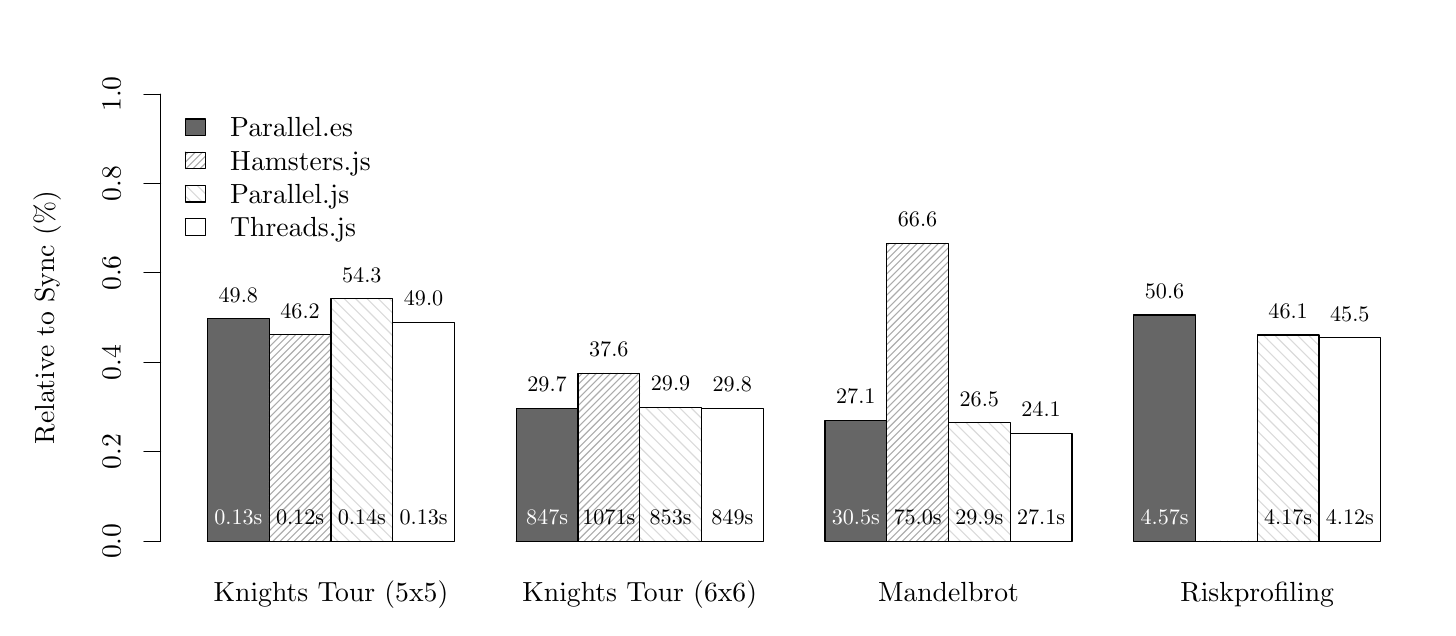
\begin{tikzpicture}[x=1pt,y=1pt]
\definecolor{fillColor}{RGB}{255,255,255}
\path[use as bounding box,fill=fillColor,fill opacity=0.00] (0,0) rectangle (505.89,209.58);
\begin{scope}
\path[clip] (  0.00,  0.00) rectangle (505.89,209.58);
\definecolor{fillColor}{gray}{0.40}

\path[fill=fillColor] ( 64.96, 24.00) --
	( 87.27, 24.00) --
	( 87.27,104.41) --
	( 64.96,104.41) --
	cycle;
\definecolor{drawColor}{RGB}{172,172,172}

\path[draw=drawColor,line width= 0.4pt,line join=round,line cap=round] ( 87.27, 96.74) -- ( 89.13, 98.59);

\path[draw=drawColor,line width= 0.4pt,line join=round,line cap=round] ( 87.27, 94.18) -- ( 91.68, 98.59);

\path[draw=drawColor,line width= 0.4pt,line join=round,line cap=round] ( 87.27, 91.62) -- ( 94.24, 98.59);

\path[draw=drawColor,line width= 0.4pt,line join=round,line cap=round] ( 87.27, 89.07) -- ( 96.79, 98.59);

\path[draw=drawColor,line width= 0.4pt,line join=round,line cap=round] ( 87.27, 86.51) -- ( 99.35, 98.59);

\path[draw=drawColor,line width= 0.4pt,line join=round,line cap=round] ( 87.27, 83.96) -- (101.90, 98.59);

\path[draw=drawColor,line width= 0.4pt,line join=round,line cap=round] ( 87.27, 81.40) -- (104.46, 98.59);

\path[draw=drawColor,line width= 0.4pt,line join=round,line cap=round] ( 87.27, 78.85) -- (107.01, 98.59);

\path[draw=drawColor,line width= 0.4pt,line join=round,line cap=round] ( 87.27, 76.29) -- (109.57, 98.59);

\path[draw=drawColor,line width= 0.4pt,line join=round,line cap=round] ( 87.27, 73.74) -- (109.59, 96.05);

\path[draw=drawColor,line width= 0.4pt,line join=round,line cap=round] ( 87.27, 71.18) -- (109.59, 93.50);

\path[draw=drawColor,line width= 0.4pt,line join=round,line cap=round] ( 87.27, 68.63) -- (109.59, 90.94);

\path[draw=drawColor,line width= 0.4pt,line join=round,line cap=round] ( 87.27, 66.07) -- (109.59, 88.39);

\path[draw=drawColor,line width= 0.4pt,line join=round,line cap=round] ( 87.27, 63.52) -- (109.59, 85.83);

\path[draw=drawColor,line width= 0.4pt,line join=round,line cap=round] ( 87.27, 60.96) -- (109.59, 83.28);

\path[draw=drawColor,line width= 0.4pt,line join=round,line cap=round] ( 87.27, 58.41) -- (109.59, 80.72);

\path[draw=drawColor,line width= 0.4pt,line join=round,line cap=round] ( 87.27, 55.85) -- (109.59, 78.17);

\path[draw=drawColor,line width= 0.4pt,line join=round,line cap=round] ( 87.27, 53.30) -- (109.59, 75.61);

\path[draw=drawColor,line width= 0.4pt,line join=round,line cap=round] ( 87.27, 50.74) -- (109.59, 73.06);

\path[draw=drawColor,line width= 0.4pt,line join=round,line cap=round] ( 87.27, 48.19) -- (109.59, 70.50);

\path[draw=drawColor,line width= 0.4pt,line join=round,line cap=round] ( 87.27, 45.63) -- (109.59, 67.95);

\path[draw=drawColor,line width= 0.4pt,line join=round,line cap=round] ( 87.27, 43.08) -- (109.59, 65.39);

\path[draw=drawColor,line width= 0.4pt,line join=round,line cap=round] ( 87.27, 40.52) -- (109.59, 62.84);

\path[draw=drawColor,line width= 0.4pt,line join=round,line cap=round] ( 87.27, 37.97) -- (109.59, 60.28);

\path[draw=drawColor,line width= 0.4pt,line join=round,line cap=round] ( 87.27, 35.41) -- (109.59, 57.73);

\path[draw=drawColor,line width= 0.4pt,line join=round,line cap=round] ( 87.27, 32.86) -- (109.59, 55.17);

\path[draw=drawColor,line width= 0.4pt,line join=round,line cap=round] ( 87.27, 30.30) -- (109.59, 52.62);

\path[draw=drawColor,line width= 0.4pt,line join=round,line cap=round] ( 87.27, 27.75) -- (109.59, 50.06);

\path[draw=drawColor,line width= 0.4pt,line join=round,line cap=round] ( 87.27, 25.19) -- (109.59, 47.51);

\path[draw=drawColor,line width= 0.4pt,line join=round,line cap=round] ( 88.64, 24.00) -- (109.59, 44.95);

\path[draw=drawColor,line width= 0.4pt,line join=round,line cap=round] ( 91.19, 24.00) -- (109.59, 42.40);

\path[draw=drawColor,line width= 0.4pt,line join=round,line cap=round] ( 93.75, 24.00) -- (109.59, 39.84);

\path[draw=drawColor,line width= 0.4pt,line join=round,line cap=round] ( 96.30, 24.00) -- (109.59, 37.29);

\path[draw=drawColor,line width= 0.4pt,line join=round,line cap=round] ( 98.86, 24.00) -- (109.59, 34.73);

\path[draw=drawColor,line width= 0.4pt,line join=round,line cap=round] (101.41, 24.00) -- (109.59, 32.17);

\path[draw=drawColor,line width= 0.4pt,line join=round,line cap=round] (103.97, 24.00) -- (109.59, 29.62);

\path[draw=drawColor,line width= 0.4pt,line join=round,line cap=round] (106.52, 24.00) -- (109.59, 27.06);

\path[draw=drawColor,line width= 0.4pt,line join=round,line cap=round] (109.08, 24.00) -- (109.59, 24.51);
\definecolor{drawColor}{RGB}{218,218,218}

\path[draw=drawColor,line width= 0.4pt,line join=round,line cap=round] (112.14, 24.00) -- (109.59, 26.56);

\path[draw=drawColor,line width= 0.4pt,line join=round,line cap=round] (116.23, 24.00) -- (109.59, 30.64);

\path[draw=drawColor,line width= 0.4pt,line join=round,line cap=round] (120.32, 24.00) -- (109.59, 34.73);

\path[draw=drawColor,line width= 0.4pt,line join=round,line cap=round] (124.41, 24.00) -- (109.59, 38.82);

\path[draw=drawColor,line width= 0.4pt,line join=round,line cap=round] (128.50, 24.00) -- (109.59, 42.91);

\path[draw=drawColor,line width= 0.4pt,line join=round,line cap=round] (131.90, 24.68) -- (109.59, 47.00);

\path[draw=drawColor,line width= 0.4pt,line join=round,line cap=round] (131.90, 28.77) -- (109.59, 51.09);

\path[draw=drawColor,line width= 0.4pt,line join=round,line cap=round] (131.90, 32.86) -- (109.59, 55.17);

\path[draw=drawColor,line width= 0.4pt,line join=round,line cap=round] (131.90, 36.95) -- (109.59, 59.26);

\path[draw=drawColor,line width= 0.4pt,line join=round,line cap=round] (131.90, 41.04) -- (109.59, 63.35);

\path[draw=drawColor,line width= 0.4pt,line join=round,line cap=round] (131.90, 45.12) -- (109.59, 67.44);

\path[draw=drawColor,line width= 0.4pt,line join=round,line cap=round] (131.90, 49.21) -- (109.59, 71.53);

\path[draw=drawColor,line width= 0.4pt,line join=round,line cap=round] (131.90, 53.30) -- (109.59, 75.62);

\path[draw=drawColor,line width= 0.4pt,line join=round,line cap=round] (131.90, 57.39) -- (109.59, 79.70);

\path[draw=drawColor,line width= 0.4pt,line join=round,line cap=round] (131.90, 61.48) -- (109.59, 83.79);

\path[draw=drawColor,line width= 0.4pt,line join=round,line cap=round] (131.90, 65.57) -- (109.59, 87.88);

\path[draw=drawColor,line width= 0.4pt,line join=round,line cap=round] (131.90, 69.65) -- (109.59, 91.97);

\path[draw=drawColor,line width= 0.4pt,line join=round,line cap=round] (131.90, 73.74) -- (109.59, 96.06);

\path[draw=drawColor,line width= 0.4pt,line join=round,line cap=round] (131.90, 77.83) -- (109.59,100.14);

\path[draw=drawColor,line width= 0.4pt,line join=round,line cap=round] (131.90, 81.92) -- (109.59,104.23);

\path[draw=drawColor,line width= 0.4pt,line join=round,line cap=round] (131.90, 86.01) -- (109.59,108.32);

\path[draw=drawColor,line width= 0.4pt,line join=round,line cap=round] (131.90, 90.09) -- (110.33,111.67);

\path[draw=drawColor,line width= 0.4pt,line join=round,line cap=round] (131.90, 94.18) -- (114.42,111.67);

\path[draw=drawColor,line width= 0.4pt,line join=round,line cap=round] (131.90, 98.27) -- (118.50,111.67);

\path[draw=drawColor,line width= 0.4pt,line join=round,line cap=round] (131.90,102.36) -- (122.59,111.67);

\path[draw=drawColor,line width= 0.4pt,line join=round,line cap=round] (131.90,106.45) -- (126.68,111.67);

\path[draw=drawColor,line width= 0.4pt,line join=round,line cap=round] (131.90,110.54) -- (130.77,111.67);

\path[fill=fillColor] (176.53, 24.00) --
	(198.84, 24.00) --
	(198.84, 71.98) --
	(176.53, 71.98) --
	cycle;
\definecolor{drawColor}{RGB}{172,172,172}

\path[draw=drawColor,line width= 0.4pt,line join=round,line cap=round] (198.84, 83.11) -- (200.43, 84.69);

\path[draw=drawColor,line width= 0.4pt,line join=round,line cap=round] (198.84, 80.55) -- (202.98, 84.69);

\path[draw=drawColor,line width= 0.4pt,line join=round,line cap=round] (198.84, 78.00) -- (205.54, 84.69);

\path[draw=drawColor,line width= 0.4pt,line join=round,line cap=round] (198.84, 75.44) -- (208.09, 84.69);

\path[draw=drawColor,line width= 0.4pt,line join=round,line cap=round] (198.84, 72.88) -- (210.65, 84.69);

\path[draw=drawColor,line width= 0.4pt,line join=round,line cap=round] (198.84, 70.33) -- (213.20, 84.69);

\path[draw=drawColor,line width= 0.4pt,line join=round,line cap=round] (198.84, 67.77) -- (215.76, 84.69);

\path[draw=drawColor,line width= 0.4pt,line join=round,line cap=round] (198.84, 65.22) -- (218.31, 84.69);

\path[draw=drawColor,line width= 0.4pt,line join=round,line cap=round] (198.84, 62.66) -- (220.87, 84.69);

\path[draw=drawColor,line width= 0.4pt,line join=round,line cap=round] (198.84, 60.11) -- (221.16, 82.42);

\path[draw=drawColor,line width= 0.4pt,line join=round,line cap=round] (198.84, 57.55) -- (221.16, 79.87);

\path[draw=drawColor,line width= 0.4pt,line join=round,line cap=round] (198.84, 55.00) -- (221.16, 77.31);

\path[draw=drawColor,line width= 0.4pt,line join=round,line cap=round] (198.84, 52.44) -- (221.16, 74.76);

\path[draw=drawColor,line width= 0.4pt,line join=round,line cap=round] (198.84, 49.89) -- (221.16, 72.20);

\path[draw=drawColor,line width= 0.4pt,line join=round,line cap=round] (198.84, 47.33) -- (221.16, 69.65);

\path[draw=drawColor,line width= 0.4pt,line join=round,line cap=round] (198.84, 44.78) -- (221.16, 67.09);

\path[draw=drawColor,line width= 0.4pt,line join=round,line cap=round] (198.84, 42.22) -- (221.16, 64.54);

\path[draw=drawColor,line width= 0.4pt,line join=round,line cap=round] (198.84, 39.67) -- (221.16, 61.98);

\path[draw=drawColor,line width= 0.4pt,line join=round,line cap=round] (198.84, 37.11) -- (221.16, 59.43);

\path[draw=drawColor,line width= 0.4pt,line join=round,line cap=round] (198.84, 34.56) -- (221.16, 56.87);

\path[draw=drawColor,line width= 0.4pt,line join=round,line cap=round] (198.84, 32.00) -- (221.16, 54.32);

\path[draw=drawColor,line width= 0.4pt,line join=round,line cap=round] (198.84, 29.45) -- (221.16, 51.76);

\path[draw=drawColor,line width= 0.4pt,line join=round,line cap=round] (198.84, 26.89) -- (221.16, 49.21);

\path[draw=drawColor,line width= 0.4pt,line join=round,line cap=round] (198.84, 24.34) -- (221.16, 46.65);

\path[draw=drawColor,line width= 0.4pt,line join=round,line cap=round] (201.06, 24.00) -- (221.16, 44.10);

\path[draw=drawColor,line width= 0.4pt,line join=round,line cap=round] (203.62, 24.00) -- (221.16, 41.54);

\path[draw=drawColor,line width= 0.4pt,line join=round,line cap=round] (206.17, 24.00) -- (221.16, 38.99);

\path[draw=drawColor,line width= 0.4pt,line join=round,line cap=round] (208.73, 24.00) -- (221.16, 36.43);

\path[draw=drawColor,line width= 0.4pt,line join=round,line cap=round] (211.28, 24.00) -- (221.16, 33.88);

\path[draw=drawColor,line width= 0.4pt,line join=round,line cap=round] (213.84, 24.00) -- (221.16, 31.32);

\path[draw=drawColor,line width= 0.4pt,line join=round,line cap=round] (216.39, 24.00) -- (221.16, 28.77);

\path[draw=drawColor,line width= 0.4pt,line join=round,line cap=round] (218.95, 24.00) -- (221.16, 26.21);
\definecolor{drawColor}{RGB}{218,218,218}

\path[draw=drawColor,line width= 0.4pt,line join=round,line cap=round] (222.53, 24.00) -- (221.16, 25.37);

\path[draw=drawColor,line width= 0.4pt,line join=round,line cap=round] (226.61, 24.00) -- (221.16, 29.45);

\path[draw=drawColor,line width= 0.4pt,line join=round,line cap=round] (230.70, 24.00) -- (221.16, 33.54);

\path[draw=drawColor,line width= 0.4pt,line join=round,line cap=round] (234.79, 24.00) -- (221.16, 37.63);

\path[draw=drawColor,line width= 0.4pt,line join=round,line cap=round] (238.88, 24.00) -- (221.16, 41.72);

\path[draw=drawColor,line width= 0.4pt,line join=round,line cap=round] (242.97, 24.00) -- (221.16, 45.81);

\path[draw=drawColor,line width= 0.4pt,line join=round,line cap=round] (243.47, 27.58) -- (221.16, 49.90);

\path[draw=drawColor,line width= 0.4pt,line join=round,line cap=round] (243.47, 31.67) -- (221.16, 53.98);

\path[draw=drawColor,line width= 0.4pt,line join=round,line cap=round] (243.47, 35.76) -- (221.16, 58.07);

\path[draw=drawColor,line width= 0.4pt,line join=round,line cap=round] (243.47, 39.85) -- (221.16, 62.16);

\path[draw=drawColor,line width= 0.4pt,line join=round,line cap=round] (243.47, 43.93) -- (221.16, 66.25);

\path[draw=drawColor,line width= 0.4pt,line join=round,line cap=round] (243.47, 48.02) -- (221.16, 70.34);

\path[draw=drawColor,line width= 0.4pt,line join=round,line cap=round] (243.47, 52.11) -- (223.24, 72.34);

\path[draw=drawColor,line width= 0.4pt,line join=round,line cap=round] (243.47, 56.20) -- (227.33, 72.34);

\path[draw=drawColor,line width= 0.4pt,line join=round,line cap=round] (243.47, 60.29) -- (231.42, 72.34);

\path[draw=drawColor,line width= 0.4pt,line join=round,line cap=round] (243.47, 64.38) -- (235.51, 72.34);

\path[draw=drawColor,line width= 0.4pt,line join=round,line cap=round] (243.47, 68.46) -- (239.60, 72.34);

\path[fill=fillColor] (288.10, 24.00) --
	(310.42, 24.00) --
	(310.42, 67.73) --
	(288.10, 67.73) --
	cycle;
\definecolor{drawColor}{RGB}{172,172,172}

\path[draw=drawColor,line width= 0.4pt,line join=round,line cap=round] (310.42,130.80) -- (311.25,131.63);

\path[draw=drawColor,line width= 0.4pt,line join=round,line cap=round] (310.42,128.24) -- (313.80,131.63);

\path[draw=drawColor,line width= 0.4pt,line join=round,line cap=round] (310.42,125.69) -- (316.36,131.63);

\path[draw=drawColor,line width= 0.4pt,line join=round,line cap=round] (310.42,123.13) -- (318.91,131.63);

\path[draw=drawColor,line width= 0.4pt,line join=round,line cap=round] (310.42,120.58) -- (321.47,131.63);

\path[draw=drawColor,line width= 0.4pt,line join=round,line cap=round] (310.42,118.02) -- (324.02,131.63);

\path[draw=drawColor,line width= 0.4pt,line join=round,line cap=round] (310.42,115.47) -- (326.58,131.63);

\path[draw=drawColor,line width= 0.4pt,line join=round,line cap=round] (310.42,112.91) -- (329.13,131.63);

\path[draw=drawColor,line width= 0.4pt,line join=round,line cap=round] (310.42,110.36) -- (331.69,131.63);

\path[draw=drawColor,line width= 0.4pt,line join=round,line cap=round] (310.42,107.80) -- (332.73,130.12);

\path[draw=drawColor,line width= 0.4pt,line join=round,line cap=round] (310.42,105.25) -- (332.73,127.56);

\path[draw=drawColor,line width= 0.4pt,line join=round,line cap=round] (310.42,102.69) -- (332.73,125.01);

\path[draw=drawColor,line width= 0.4pt,line join=round,line cap=round] (310.42,100.14) -- (332.73,122.45);

\path[draw=drawColor,line width= 0.4pt,line join=round,line cap=round] (310.42, 97.58) -- (332.73,119.90);

\path[draw=drawColor,line width= 0.4pt,line join=round,line cap=round] (310.42, 95.03) -- (332.73,117.34);

\path[draw=drawColor,line width= 0.4pt,line join=round,line cap=round] (310.42, 92.47) -- (332.73,114.79);

\path[draw=drawColor,line width= 0.4pt,line join=round,line cap=round] (310.42, 89.92) -- (332.73,112.23);

\path[draw=drawColor,line width= 0.4pt,line join=round,line cap=round] (310.42, 87.36) -- (332.73,109.68);

\path[draw=drawColor,line width= 0.4pt,line join=round,line cap=round] (310.42, 84.81) -- (332.73,107.12);

\path[draw=drawColor,line width= 0.4pt,line join=round,line cap=round] (310.42, 82.25) -- (332.73,104.57);

\path[draw=drawColor,line width= 0.4pt,line join=round,line cap=round] (310.42, 79.70) -- (332.73,102.01);

\path[draw=drawColor,line width= 0.4pt,line join=round,line cap=round] (310.42, 77.14) -- (332.73, 99.46);

\path[draw=drawColor,line width= 0.4pt,line join=round,line cap=round] (310.42, 74.59) -- (332.73, 96.90);

\path[draw=drawColor,line width= 0.4pt,line join=round,line cap=round] (310.42, 72.03) -- (332.73, 94.35);

\path[draw=drawColor,line width= 0.4pt,line join=round,line cap=round] (310.42, 69.48) -- (332.73, 91.79);

\path[draw=drawColor,line width= 0.4pt,line join=round,line cap=round] (310.42, 66.92) -- (332.73, 89.23);

\path[draw=drawColor,line width= 0.4pt,line join=round,line cap=round] (310.42, 64.37) -- (332.73, 86.68);

\path[draw=drawColor,line width= 0.4pt,line join=round,line cap=round] (310.42, 61.81) -- (332.73, 84.12);

\path[draw=drawColor,line width= 0.4pt,line join=round,line cap=round] (310.42, 59.26) -- (332.73, 81.57);

\path[draw=drawColor,line width= 0.4pt,line join=round,line cap=round] (310.42, 56.70) -- (332.73, 79.01);

\path[draw=drawColor,line width= 0.4pt,line join=round,line cap=round] (310.42, 54.14) -- (332.73, 76.46);

\path[draw=drawColor,line width= 0.4pt,line join=round,line cap=round] (310.42, 51.59) -- (332.73, 73.90);

\path[draw=drawColor,line width= 0.4pt,line join=round,line cap=round] (310.42, 49.03) -- (332.73, 71.35);

\path[draw=drawColor,line width= 0.4pt,line join=round,line cap=round] (310.42, 46.48) -- (332.73, 68.79);

\path[draw=drawColor,line width= 0.4pt,line join=round,line cap=round] (310.42, 43.92) -- (332.73, 66.24);

\path[draw=drawColor,line width= 0.4pt,line join=round,line cap=round] (310.42, 41.37) -- (332.73, 63.68);

\path[draw=drawColor,line width= 0.4pt,line join=round,line cap=round] (310.42, 38.81) -- (332.73, 61.13);

\path[draw=drawColor,line width= 0.4pt,line join=round,line cap=round] (310.42, 36.26) -- (332.73, 58.57);

\path[draw=drawColor,line width= 0.4pt,line join=round,line cap=round] (310.42, 33.70) -- (332.73, 56.02);

\path[draw=drawColor,line width= 0.4pt,line join=round,line cap=round] (310.42, 31.15) -- (332.73, 53.46);

\path[draw=drawColor,line width= 0.4pt,line join=round,line cap=round] (310.42, 28.59) -- (332.73, 50.91);

\path[draw=drawColor,line width= 0.4pt,line join=round,line cap=round] (310.42, 26.04) -- (332.73, 48.35);

\path[draw=drawColor,line width= 0.4pt,line join=round,line cap=round] (310.93, 24.00) -- (332.73, 45.80);

\path[draw=drawColor,line width= 0.4pt,line join=round,line cap=round] (313.49, 24.00) -- (332.73, 43.24);

\path[draw=drawColor,line width= 0.4pt,line join=round,line cap=round] (316.04, 24.00) -- (332.73, 40.69);

\path[draw=drawColor,line width= 0.4pt,line join=round,line cap=round] (318.60, 24.00) -- (332.73, 38.13);

\path[draw=drawColor,line width= 0.4pt,line join=round,line cap=round] (321.15, 24.00) -- (332.73, 35.58);

\path[draw=drawColor,line width= 0.4pt,line join=round,line cap=round] (323.71, 24.00) -- (332.73, 33.02);

\path[draw=drawColor,line width= 0.4pt,line join=round,line cap=round] (326.26, 24.00) -- (332.73, 30.47);

\path[draw=drawColor,line width= 0.4pt,line join=round,line cap=round] (328.82, 24.00) -- (332.73, 27.91);

\path[draw=drawColor,line width= 0.4pt,line join=round,line cap=round] (331.37, 24.00) -- (332.73, 25.36);
\definecolor{drawColor}{RGB}{218,218,218}

\path[draw=drawColor,line width= 0.4pt,line join=round,line cap=round] (332.91, 24.00) -- (332.73, 24.18);

\path[draw=drawColor,line width= 0.4pt,line join=round,line cap=round] (337.00, 24.00) -- (332.73, 28.26);

\path[draw=drawColor,line width= 0.4pt,line join=round,line cap=round] (341.08, 24.00) -- (332.73, 32.35);

\path[draw=drawColor,line width= 0.4pt,line join=round,line cap=round] (345.17, 24.00) -- (332.73, 36.44);

\path[draw=drawColor,line width= 0.4pt,line join=round,line cap=round] (349.26, 24.00) -- (332.73, 40.53);

\path[draw=drawColor,line width= 0.4pt,line join=round,line cap=round] (353.35, 24.00) -- (332.73, 44.62);

\path[draw=drawColor,line width= 0.4pt,line join=round,line cap=round] (355.05, 26.39) -- (332.73, 48.71);

\path[draw=drawColor,line width= 0.4pt,line join=round,line cap=round] (355.05, 30.48) -- (332.73, 52.79);

\path[draw=drawColor,line width= 0.4pt,line join=round,line cap=round] (355.05, 34.57) -- (332.73, 56.88);

\path[draw=drawColor,line width= 0.4pt,line join=round,line cap=round] (355.05, 38.66) -- (332.73, 60.97);

\path[draw=drawColor,line width= 0.4pt,line join=round,line cap=round] (355.05, 42.74) -- (332.73, 65.06);

\path[draw=drawColor,line width= 0.4pt,line join=round,line cap=round] (355.05, 46.83) -- (335.03, 66.85);

\path[draw=drawColor,line width= 0.4pt,line join=round,line cap=round] (355.05, 50.92) -- (339.12, 66.85);

\path[draw=drawColor,line width= 0.4pt,line join=round,line cap=round] (355.05, 55.01) -- (343.21, 66.85);

\path[draw=drawColor,line width= 0.4pt,line join=round,line cap=round] (355.05, 59.10) -- (347.30, 66.85);

\path[draw=drawColor,line width= 0.4pt,line join=round,line cap=round] (355.05, 63.19) -- (351.38, 66.85);

\path[fill=fillColor] (399.67, 24.00) --
	(421.99, 24.00) --
	(421.99,105.75) --
	(399.67,105.75) --
	cycle;
\definecolor{drawColor}{RGB}{172,172,172}

\path[draw=drawColor,line width= 0.4pt,line join=round,line cap=round] (423.36, 24.00) -- (423.36, 24.00);

\path[draw=drawColor,line width= 0.4pt,line join=round,line cap=round] (425.91, 24.00) -- (425.91, 24.00);

\path[draw=drawColor,line width= 0.4pt,line join=round,line cap=round] (428.47, 24.00) -- (428.47, 24.00);

\path[draw=drawColor,line width= 0.4pt,line join=round,line cap=round] (431.02, 24.00) -- (431.02, 24.00);

\path[draw=drawColor,line width= 0.4pt,line join=round,line cap=round] (433.58, 24.00) -- (433.58, 24.00);

\path[draw=drawColor,line width= 0.4pt,line join=round,line cap=round] (436.13, 24.00) -- (436.13, 24.00);

\path[draw=drawColor,line width= 0.4pt,line join=round,line cap=round] (438.69, 24.00) -- (438.69, 24.00);

\path[draw=drawColor,line width= 0.4pt,line join=round,line cap=round] (441.24, 24.00) -- (441.24, 24.00);

\path[draw=drawColor,line width= 0.4pt,line join=round,line cap=round] (443.80, 24.00) -- (443.80, 24.00);
\definecolor{drawColor}{RGB}{218,218,218}

\path[draw=drawColor,line width= 0.4pt,line join=round,line cap=round] (447.38, 24.00) -- (444.30, 27.07);

\path[draw=drawColor,line width= 0.4pt,line join=round,line cap=round] (451.47, 24.00) -- (444.30, 31.16);

\path[draw=drawColor,line width= 0.4pt,line join=round,line cap=round] (455.55, 24.00) -- (444.30, 35.25);

\path[draw=drawColor,line width= 0.4pt,line join=round,line cap=round] (459.64, 24.00) -- (444.30, 39.34);

\path[draw=drawColor,line width= 0.4pt,line join=round,line cap=round] (463.73, 24.00) -- (444.30, 43.43);

\path[draw=drawColor,line width= 0.4pt,line join=round,line cap=round] (466.62, 25.20) -- (444.30, 47.52);

\path[draw=drawColor,line width= 0.4pt,line join=round,line cap=round] (466.62, 29.29) -- (444.30, 51.60);

\path[draw=drawColor,line width= 0.4pt,line join=round,line cap=round] (466.62, 33.38) -- (444.30, 55.69);

\path[draw=drawColor,line width= 0.4pt,line join=round,line cap=round] (466.62, 37.47) -- (444.30, 59.78);

\path[draw=drawColor,line width= 0.4pt,line join=round,line cap=round] (466.62, 41.55) -- (444.30, 63.87);

\path[draw=drawColor,line width= 0.4pt,line join=round,line cap=round] (466.62, 45.64) -- (444.30, 67.96);

\path[draw=drawColor,line width= 0.4pt,line join=round,line cap=round] (466.62, 49.73) -- (444.30, 72.05);

\path[draw=drawColor,line width= 0.4pt,line join=round,line cap=round] (466.62, 53.82) -- (444.30, 76.13);

\path[draw=drawColor,line width= 0.4pt,line join=round,line cap=round] (466.62, 57.91) -- (444.30, 80.22);

\path[draw=drawColor,line width= 0.4pt,line join=round,line cap=round] (466.62, 62.00) -- (444.30, 84.31);

\path[draw=drawColor,line width= 0.4pt,line join=round,line cap=round] (466.62, 66.08) -- (444.30, 88.40);

\path[draw=drawColor,line width= 0.4pt,line join=round,line cap=round] (466.62, 70.17) -- (444.30, 92.49);

\path[draw=drawColor,line width= 0.4pt,line join=round,line cap=round] (466.62, 74.26) -- (444.30, 96.57);

\path[draw=drawColor,line width= 0.4pt,line join=round,line cap=round] (466.62, 78.35) -- (446.43, 98.53);

\path[draw=drawColor,line width= 0.4pt,line join=round,line cap=round] (466.62, 82.44) -- (450.52, 98.53);

\path[draw=drawColor,line width= 0.4pt,line join=round,line cap=round] (466.62, 86.52) -- (454.61, 98.53);

\path[draw=drawColor,line width= 0.4pt,line join=round,line cap=round] (466.62, 90.61) -- (458.70, 98.53);

\path[draw=drawColor,line width= 0.4pt,line join=round,line cap=round] (466.62, 94.70) -- (462.78, 98.53);
\definecolor{drawColor}{RGB}{0,0,0}

\path[draw=drawColor,line width= 0.4pt,line join=round,line cap=round] ( 64.96, 24.00) --
	( 87.27, 24.00) --
	( 87.27,104.41) --
	( 64.96,104.41) --
	( 64.96, 24.00);

\path[draw=drawColor,line width= 0.4pt,line join=round,line cap=round] ( 87.27, 24.00) --
	(109.59, 24.00) --
	(109.59, 98.59) --
	( 87.27, 98.59) --
	( 87.27, 24.00);

\path[draw=drawColor,line width= 0.4pt,line join=round,line cap=round] (109.59, 24.00) --
	(131.90, 24.00) --
	(131.90,111.67) --
	(109.59,111.67) --
	(109.59, 24.00);

\path[draw=drawColor,line width= 0.4pt,line join=round,line cap=round] (131.90, 24.00) --
	(154.22, 24.00) --
	(154.22,103.12) --
	(131.90,103.12) --
	(131.90, 24.00);

\path[draw=drawColor,line width= 0.4pt,line join=round,line cap=round] (176.53, 24.00) --
	(198.84, 24.00) --
	(198.84, 71.98) --
	(176.53, 71.98) --
	(176.53, 24.00);

\path[draw=drawColor,line width= 0.4pt,line join=round,line cap=round] (198.84, 24.00) --
	(221.16, 24.00) --
	(221.16, 84.69) --
	(198.84, 84.69) --
	(198.84, 24.00);

\path[draw=drawColor,line width= 0.4pt,line join=round,line cap=round] (221.16, 24.00) --
	(243.47, 24.00) --
	(243.47, 72.34) --
	(221.16, 72.34) --
	(221.16, 24.00);

\path[draw=drawColor,line width= 0.4pt,line join=round,line cap=round] (243.47, 24.00) --
	(265.79, 24.00) --
	(265.79, 72.09) --
	(243.47, 72.09) --
	(243.47, 24.00);

\path[draw=drawColor,line width= 0.4pt,line join=round,line cap=round] (288.10, 24.00) --
	(310.42, 24.00) --
	(310.42, 67.73) --
	(288.10, 67.73) --
	(288.10, 24.00);

\path[draw=drawColor,line width= 0.4pt,line join=round,line cap=round] (310.42, 24.00) --
	(332.73, 24.00) --
	(332.73,131.63) --
	(310.42,131.63) --
	(310.42, 24.00);

\path[draw=drawColor,line width= 0.4pt,line join=round,line cap=round] (332.73, 24.00) --
	(355.05, 24.00) --
	(355.05, 66.85) --
	(332.73, 66.85) --
	(332.73, 24.00);

\path[draw=drawColor,line width= 0.4pt,line join=round,line cap=round] (355.05, 24.00) --
	(377.36, 24.00) --
	(377.36, 62.92) --
	(355.05, 62.92) --
	(355.05, 24.00);

\path[draw=drawColor,line width= 0.4pt,line join=round,line cap=round] (399.67, 24.00) --
	(421.99, 24.00) --
	(421.99,105.75) --
	(399.67,105.75) --
	(399.67, 24.00);

\path[draw=drawColor,line width= 0.4pt,line join=round,line cap=round] (421.99, 24.00) --
	(444.30, 24.00) --
	(421.99, 24.00);

\path[draw=drawColor,line width= 0.4pt,line join=round,line cap=round] (444.30, 24.00) --
	(466.62, 24.00) --
	(466.62, 98.53) --
	(444.30, 98.53) --
	(444.30, 24.00);

\path[draw=drawColor,line width= 0.4pt,line join=round,line cap=round] (466.62, 24.00) --
	(488.93, 24.00) --
	(488.93, 97.58) --
	(466.62, 97.58) --
	(466.62, 24.00);
\end{scope}
\begin{scope}
\path[clip] (  0.00,  0.00) rectangle (505.89,209.58);
\definecolor{drawColor}{RGB}{0,0,0}

\node[text=drawColor,anchor=base,inner sep=0pt, outer sep=0pt, scale=  1.00] at (109.59,  2.40) {Knights Tour (5x5)};

\node[text=drawColor,anchor=base,inner sep=0pt, outer sep=0pt, scale=  1.00] at (221.16,  2.40) {Knights Tour (6x6)};

\node[text=drawColor,anchor=base,inner sep=0pt, outer sep=0pt, scale=  1.00] at (332.73,  2.40) {Mandelbrot};

\node[text=drawColor,anchor=base,inner sep=0pt, outer sep=0pt, scale=  1.00] at (444.30,  2.40) {Riskprofiling};
\end{scope}
\begin{scope}
\path[clip] (  0.00,  0.00) rectangle (505.89,209.58);
\definecolor{drawColor}{RGB}{0,0,0}

\node[text=drawColor,rotate= 90.00,anchor=base,inner sep=0pt, outer sep=0pt, scale=  1.00] at (  9.60,104.79) {Relative to Sync ({\%})};
\end{scope}
\begin{scope}
\path[clip] (  0.00,  0.00) rectangle (505.89,209.58);
\definecolor{drawColor}{RGB}{0,0,0}

\path[draw=drawColor,line width= 0.4pt,line join=round,line cap=round] ( 48.00, 24.00) -- ( 48.00,185.58);

\path[draw=drawColor,line width= 0.4pt,line join=round,line cap=round] ( 48.00, 24.00) -- ( 42.00, 24.00);

\path[draw=drawColor,line width= 0.4pt,line join=round,line cap=round] ( 48.00, 56.32) -- ( 42.00, 56.32);

\path[draw=drawColor,line width= 0.4pt,line join=round,line cap=round] ( 48.00, 88.63) -- ( 42.00, 88.63);

\path[draw=drawColor,line width= 0.4pt,line join=round,line cap=round] ( 48.00,120.95) -- ( 42.00,120.95);

\path[draw=drawColor,line width= 0.4pt,line join=round,line cap=round] ( 48.00,153.27) -- ( 42.00,153.27);

\path[draw=drawColor,line width= 0.4pt,line join=round,line cap=round] ( 48.00,185.58) -- ( 42.00,185.58);

\node[text=drawColor,rotate= 90.00,anchor=base,inner sep=0pt, outer sep=0pt, scale=  1.00] at ( 33.60, 24.00) {0.0};

\node[text=drawColor,rotate= 90.00,anchor=base,inner sep=0pt, outer sep=0pt, scale=  1.00] at ( 33.60, 56.32) {0.2};

\node[text=drawColor,rotate= 90.00,anchor=base,inner sep=0pt, outer sep=0pt, scale=  1.00] at ( 33.60, 88.63) {0.4};

\node[text=drawColor,rotate= 90.00,anchor=base,inner sep=0pt, outer sep=0pt, scale=  1.00] at ( 33.60,120.95) {0.6};

\node[text=drawColor,rotate= 90.00,anchor=base,inner sep=0pt, outer sep=0pt, scale=  1.00] at ( 33.60,153.27) {0.8};

\node[text=drawColor,rotate= 90.00,anchor=base,inner sep=0pt, outer sep=0pt, scale=  1.00] at ( 33.60,185.58) {1.0};
\end{scope}
\begin{scope}
\path[clip] ( 48.00, 24.00) rectangle (505.89,185.58);
\definecolor{fillColor}{gray}{0.40}

\path[fill=fillColor] ( 57.00,176.58) --
	( 64.20,176.58) --
	( 64.20,170.58) --
	( 57.00,170.58) --
	cycle;
\definecolor{drawColor}{RGB}{172,172,172}

\path[draw=drawColor,line width= 0.4pt,line join=round,line cap=round] ( 57.00,163.56) -- ( 58.03,164.58);

\path[draw=drawColor,line width= 0.4pt,line join=round,line cap=round] ( 57.00,161.00) -- ( 60.58,164.58);

\path[draw=drawColor,line width= 0.4pt,line join=round,line cap=round] ( 57.14,158.58) -- ( 63.14,164.58);

\path[draw=drawColor,line width= 0.4pt,line join=round,line cap=round] ( 59.69,158.58) -- ( 64.20,163.09);

\path[draw=drawColor,line width= 0.4pt,line join=round,line cap=round] ( 62.25,158.58) -- ( 64.20,160.54);
\definecolor{drawColor}{RGB}{218,218,218}

\path[draw=drawColor,line width= 0.4pt,line join=round,line cap=round] ( 59.06,146.58) -- ( 57.00,148.64);

\path[draw=drawColor,line width= 0.4pt,line join=round,line cap=round] ( 63.15,146.58) -- ( 57.15,152.58);

\path[draw=drawColor,line width= 0.4pt,line join=round,line cap=round] ( 64.20,149.62) -- ( 61.24,152.58);
\definecolor{drawColor}{RGB}{0,0,0}

\path[draw=drawColor,line width= 0.4pt,line join=round,line cap=round] ( 57.00,176.58) --
	( 64.20,176.58) --
	( 64.20,170.58) --
	( 57.00,170.58) --
	( 57.00,176.58);

\path[draw=drawColor,line width= 0.4pt,line join=round,line cap=round] ( 57.00,164.58) --
	( 64.20,164.58) --
	( 64.20,158.58) --
	( 57.00,158.58) --
	( 57.00,164.58);

\path[draw=drawColor,line width= 0.4pt,line join=round,line cap=round] ( 57.00,152.58) --
	( 64.20,152.58) --
	( 64.20,146.58) --
	( 57.00,146.58) --
	( 57.00,152.58);

\path[draw=drawColor,line width= 0.4pt,line join=round,line cap=round] ( 57.00,140.58) --
	( 64.20,140.58) --
	( 64.20,134.58) --
	( 57.00,134.58) --
	( 57.00,140.58);

\node[text=drawColor,anchor=base west,inner sep=0pt, outer sep=0pt, scale=  1.00] at ( 73.20,170.14) {Parallel.es};

\node[text=drawColor,anchor=base west,inner sep=0pt, outer sep=0pt, scale=  1.00] at ( 73.20,158.14) {Hamsters.js};

\node[text=drawColor,anchor=base west,inner sep=0pt, outer sep=0pt, scale=  1.00] at ( 73.20,146.14) {Parallel.js};

\node[text=drawColor,anchor=base west,inner sep=0pt, outer sep=0pt, scale=  1.00] at ( 73.20,134.14) {Threads.js};

\node[text=drawColor,anchor=base,inner sep=0pt, outer sep=0pt, scale=  0.80] at ( 76.12,110.41) {49.8};

\node[text=drawColor,anchor=base,inner sep=0pt, outer sep=0pt, scale=  0.80] at ( 98.43,104.59) {46.2};

\node[text=drawColor,anchor=base,inner sep=0pt, outer sep=0pt, scale=  0.80] at (120.74,117.67) {54.3};

\node[text=drawColor,anchor=base,inner sep=0pt, outer sep=0pt, scale=  0.80] at (143.06,109.12) {49.0};

\node[text=drawColor,anchor=base,inner sep=0pt, outer sep=0pt, scale=  0.80] at (187.69, 77.98) {29.7};

\node[text=drawColor,anchor=base,inner sep=0pt, outer sep=0pt, scale=  0.80] at (210.00, 90.69) {37.6};

\node[text=drawColor,anchor=base,inner sep=0pt, outer sep=0pt, scale=  0.80] at (232.32, 78.34) {29.9};

\node[text=drawColor,anchor=base,inner sep=0pt, outer sep=0pt, scale=  0.80] at (254.63, 78.09) {29.8};

\node[text=drawColor,anchor=base,inner sep=0pt, outer sep=0pt, scale=  0.80] at (299.26, 73.73) {27.1};

\node[text=drawColor,anchor=base,inner sep=0pt, outer sep=0pt, scale=  0.80] at (321.57,137.63) {66.6};

\node[text=drawColor,anchor=base,inner sep=0pt, outer sep=0pt, scale=  0.80] at (343.89, 72.85) {26.5};

\node[text=drawColor,anchor=base,inner sep=0pt, outer sep=0pt, scale=  0.80] at (366.20, 68.92) {24.1};

\node[text=drawColor,anchor=base,inner sep=0pt, outer sep=0pt, scale=  0.80] at (410.83,111.75) {50.6};

\node[text=drawColor,anchor=base,inner sep=0pt, outer sep=0pt, scale=  0.80] at (455.46,104.53) {46.1};

\node[text=drawColor,anchor=base,inner sep=0pt, outer sep=0pt, scale=  0.80] at (477.77,103.58) {45.5};
\definecolor{drawColor}{RGB}{255,255,255}

\node[text=drawColor,anchor=base,inner sep=0pt, outer sep=0pt, scale=  0.80] at ( 76.12, 30.00) {0.13s};
\definecolor{drawColor}{RGB}{0,0,0}

\node[text=drawColor,anchor=base,inner sep=0pt, outer sep=0pt, scale=  0.80] at ( 98.43, 30.00) {0.12s};

\node[text=drawColor,anchor=base,inner sep=0pt, outer sep=0pt, scale=  0.80] at (120.74, 30.00) {0.14s};

\node[text=drawColor,anchor=base,inner sep=0pt, outer sep=0pt, scale=  0.80] at (143.06, 30.00) {0.13s};
\definecolor{drawColor}{RGB}{255,255,255}

\node[text=drawColor,anchor=base,inner sep=0pt, outer sep=0pt, scale=  0.80] at (187.69, 30.00) {847s};
\definecolor{drawColor}{RGB}{0,0,0}

\node[text=drawColor,anchor=base,inner sep=0pt, outer sep=0pt, scale=  0.80] at (210.00, 30.00) {1071s};

\node[text=drawColor,anchor=base,inner sep=0pt, outer sep=0pt, scale=  0.80] at (232.32, 30.00) {853s};

\node[text=drawColor,anchor=base,inner sep=0pt, outer sep=0pt, scale=  0.80] at (254.63, 30.00) {849s};
\definecolor{drawColor}{RGB}{255,255,255}

\node[text=drawColor,anchor=base,inner sep=0pt, outer sep=0pt, scale=  0.80] at (299.26, 30.00) {30.5s};
\definecolor{drawColor}{RGB}{0,0,0}

\node[text=drawColor,anchor=base,inner sep=0pt, outer sep=0pt, scale=  0.80] at (321.57, 30.00) {75.0s};

\node[text=drawColor,anchor=base,inner sep=0pt, outer sep=0pt, scale=  0.80] at (343.89, 30.00) {29.9s};

\node[text=drawColor,anchor=base,inner sep=0pt, outer sep=0pt, scale=  0.80] at (366.20, 30.00) {27.1s};
\definecolor{drawColor}{RGB}{255,255,255}

\node[text=drawColor,anchor=base,inner sep=0pt, outer sep=0pt, scale=  0.80] at (410.83, 30.00) {4.57s};
\definecolor{drawColor}{RGB}{0,0,0}

\node[text=drawColor,anchor=base,inner sep=0pt, outer sep=0pt, scale=  0.80] at (455.46, 30.00) {4.17s};

\node[text=drawColor,anchor=base,inner sep=0pt, outer sep=0pt, scale=  0.80] at (477.77, 30.00) {4.12s};
\end{scope}
\end{tikzpicture}
	
	\caption{Runtime Performance of Parallelization Problems Relative to Synchronously Execution}
	\label{fig:runtime-performance}
\end{figure*}


\paragraph{Knight Tour} The time needed to solve the knight tour problem is mainly determined by the available computational resources. The knight tour calculation is parallelized by computing the number of tours starting from a specific start-field sequence and summarizing the  number of found tours at the end. 

Parallel.js creates new tasks for accumulating the sub-results of two start field sequences computed by two tasks and executes them on designated background threads. That results in a significant overhead for the smaller 5x5 board. However, the impact is no longer visible for the larger board where the computation of the tours takes a multitude of the accumulation overhead caused by accumulating in separate tasks.

The usage of a thread pool that avoids spawning new background threads for every task does not bring the expected performance gain. The overhead for creating background threads in Firefox seems to be very inexpensive so that the effect is not visible at all. However, the benchmarking results of Google Chrome shown in \cref{fig:runtime-performance-chrome} give evidence that a thread pool might be beneficial for very short running tasks. Thus, Hamsters.js and Parallel.es achieve slightly better results than Parallel.js, that is not using a thread pool at all, and Threads.js, where a new thread pool is created manually for each execution\footnote{A new thread pool for each run is not strictly necessary for the knight tour problem. However, it is needed to store the simulation result of the risk profiling problem.}. 

\begin{figure}
	\centering
	% Created by tikzDevice version 0.10.1 on 2016-11-27 16:52:18
% !TEX encoding = UTF-8 Unicode
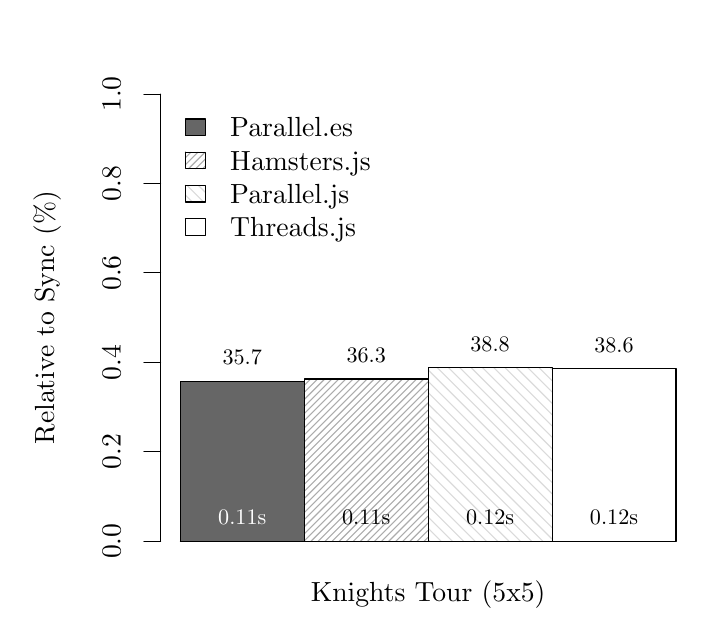
\begin{tikzpicture}[x=1pt,y=1pt]
\definecolor{fillColor}{RGB}{255,255,255}
\path[use as bounding box,fill=fillColor,fill opacity=0.00] (0,0) rectangle (241.43,209.58);
\begin{scope}
\path[clip] (  0.00,  0.00) rectangle (241.43,209.58);
\definecolor{fillColor}{gray}{0.40}

\path[fill=fillColor] ( 55.16, 24.00) --
	( 99.94, 24.00) --
	( 99.94, 81.76) --
	( 55.16, 81.76) --
	cycle;
\definecolor{drawColor}{RGB}{172,172,172}

\path[draw=drawColor,line width= 0.4pt,line join=round,line cap=round] ( 99.94, 80.33) -- (102.22, 82.61);

\path[draw=drawColor,line width= 0.4pt,line join=round,line cap=round] ( 99.94, 77.78) -- (104.77, 82.61);

\path[draw=drawColor,line width= 0.4pt,line join=round,line cap=round] ( 99.94, 75.22) -- (107.33, 82.61);

\path[draw=drawColor,line width= 0.4pt,line join=round,line cap=round] ( 99.94, 72.67) -- (109.88, 82.61);

\path[draw=drawColor,line width= 0.4pt,line join=round,line cap=round] ( 99.94, 70.11) -- (112.44, 82.61);

\path[draw=drawColor,line width= 0.4pt,line join=round,line cap=round] ( 99.94, 67.56) -- (114.99, 82.61);

\path[draw=drawColor,line width= 0.4pt,line join=round,line cap=round] ( 99.94, 65.00) -- (117.55, 82.61);

\path[draw=drawColor,line width= 0.4pt,line join=round,line cap=round] ( 99.94, 62.45) -- (120.10, 82.61);

\path[draw=drawColor,line width= 0.4pt,line join=round,line cap=round] ( 99.94, 59.89) -- (122.66, 82.61);

\path[draw=drawColor,line width= 0.4pt,line join=round,line cap=round] ( 99.94, 57.34) -- (125.21, 82.61);

\path[draw=drawColor,line width= 0.4pt,line join=round,line cap=round] ( 99.94, 54.78) -- (127.77, 82.61);

\path[draw=drawColor,line width= 0.4pt,line join=round,line cap=round] ( 99.94, 52.23) -- (130.32, 82.61);

\path[draw=drawColor,line width= 0.4pt,line join=round,line cap=round] ( 99.94, 49.67) -- (132.88, 82.61);

\path[draw=drawColor,line width= 0.4pt,line join=round,line cap=round] ( 99.94, 47.12) -- (135.43, 82.61);

\path[draw=drawColor,line width= 0.4pt,line join=round,line cap=round] ( 99.94, 44.56) -- (137.99, 82.61);

\path[draw=drawColor,line width= 0.4pt,line join=round,line cap=round] ( 99.94, 42.01) -- (140.54, 82.61);

\path[draw=drawColor,line width= 0.4pt,line join=round,line cap=round] ( 99.94, 39.45) -- (143.10, 82.61);

\path[draw=drawColor,line width= 0.4pt,line join=round,line cap=round] ( 99.94, 36.90) -- (144.71, 81.67);

\path[draw=drawColor,line width= 0.4pt,line join=round,line cap=round] ( 99.94, 34.34) -- (144.71, 79.12);

\path[draw=drawColor,line width= 0.4pt,line join=round,line cap=round] ( 99.94, 31.79) -- (144.71, 76.56);

\path[draw=drawColor,line width= 0.4pt,line join=round,line cap=round] ( 99.94, 29.23) -- (144.71, 74.01);

\path[draw=drawColor,line width= 0.4pt,line join=round,line cap=round] ( 99.94, 26.68) -- (144.71, 71.45);

\path[draw=drawColor,line width= 0.4pt,line join=round,line cap=round] ( 99.94, 24.12) -- (144.71, 68.90);

\path[draw=drawColor,line width= 0.4pt,line join=round,line cap=round] (102.37, 24.00) -- (144.71, 66.34);

\path[draw=drawColor,line width= 0.4pt,line join=round,line cap=round] (104.93, 24.00) -- (144.71, 63.79);

\path[draw=drawColor,line width= 0.4pt,line join=round,line cap=round] (107.48, 24.00) -- (144.71, 61.23);

\path[draw=drawColor,line width= 0.4pt,line join=round,line cap=round] (110.04, 24.00) -- (144.71, 58.68);

\path[draw=drawColor,line width= 0.4pt,line join=round,line cap=round] (112.59, 24.00) -- (144.71, 56.12);

\path[draw=drawColor,line width= 0.4pt,line join=round,line cap=round] (115.15, 24.00) -- (144.71, 53.57);

\path[draw=drawColor,line width= 0.4pt,line join=round,line cap=round] (117.70, 24.00) -- (144.71, 51.01);

\path[draw=drawColor,line width= 0.4pt,line join=round,line cap=round] (120.26, 24.00) -- (144.71, 48.45);

\path[draw=drawColor,line width= 0.4pt,line join=round,line cap=round] (122.81, 24.00) -- (144.71, 45.90);

\path[draw=drawColor,line width= 0.4pt,line join=round,line cap=round] (125.37, 24.00) -- (144.71, 43.34);

\path[draw=drawColor,line width= 0.4pt,line join=round,line cap=round] (127.92, 24.00) -- (144.71, 40.79);

\path[draw=drawColor,line width= 0.4pt,line join=round,line cap=round] (130.48, 24.00) -- (144.71, 38.23);

\path[draw=drawColor,line width= 0.4pt,line join=round,line cap=round] (133.04, 24.00) -- (144.71, 35.68);

\path[draw=drawColor,line width= 0.4pt,line join=round,line cap=round] (135.59, 24.00) -- (144.71, 33.12);

\path[draw=drawColor,line width= 0.4pt,line join=round,line cap=round] (138.15, 24.00) -- (144.71, 30.57);

\path[draw=drawColor,line width= 0.4pt,line join=round,line cap=round] (140.70, 24.00) -- (144.71, 28.01);

\path[draw=drawColor,line width= 0.4pt,line join=round,line cap=round] (143.26, 24.00) -- (144.71, 25.46);
\definecolor{drawColor}{RGB}{218,218,218}

\path[draw=drawColor,line width= 0.4pt,line join=round,line cap=round] (145.30, 24.00) -- (144.71, 24.59);

\path[draw=drawColor,line width= 0.4pt,line join=round,line cap=round] (149.39, 24.00) -- (144.71, 28.67);

\path[draw=drawColor,line width= 0.4pt,line join=round,line cap=round] (153.48, 24.00) -- (144.71, 32.76);

\path[draw=drawColor,line width= 0.4pt,line join=round,line cap=round] (157.56, 24.00) -- (144.71, 36.85);

\path[draw=drawColor,line width= 0.4pt,line join=round,line cap=round] (161.65, 24.00) -- (144.71, 40.94);

\path[draw=drawColor,line width= 0.4pt,line join=round,line cap=round] (165.74, 24.00) -- (144.71, 45.03);

\path[draw=drawColor,line width= 0.4pt,line join=round,line cap=round] (169.83, 24.00) -- (144.71, 49.11);

\path[draw=drawColor,line width= 0.4pt,line join=round,line cap=round] (173.92, 24.00) -- (144.71, 53.20);

\path[draw=drawColor,line width= 0.4pt,line join=round,line cap=round] (178.01, 24.00) -- (144.71, 57.29);

\path[draw=drawColor,line width= 0.4pt,line join=round,line cap=round] (182.09, 24.00) -- (144.71, 61.38);

\path[draw=drawColor,line width= 0.4pt,line join=round,line cap=round] (186.18, 24.00) -- (144.71, 65.47);

\path[draw=drawColor,line width= 0.4pt,line join=round,line cap=round] (189.49, 24.78) -- (144.71, 69.56);

\path[draw=drawColor,line width= 0.4pt,line join=round,line cap=round] (189.49, 28.87) -- (144.71, 73.64);

\path[draw=drawColor,line width= 0.4pt,line join=round,line cap=round] (189.49, 32.96) -- (144.71, 77.73);

\path[draw=drawColor,line width= 0.4pt,line join=round,line cap=round] (189.49, 37.05) -- (144.71, 81.82);

\path[draw=drawColor,line width= 0.4pt,line join=round,line cap=round] (189.49, 41.13) -- (144.71, 85.91);

\path[draw=drawColor,line width= 0.4pt,line join=round,line cap=round] (189.49, 45.22) -- (147.98, 86.73);

\path[draw=drawColor,line width= 0.4pt,line join=round,line cap=round] (189.49, 49.31) -- (152.07, 86.73);

\path[draw=drawColor,line width= 0.4pt,line join=round,line cap=round] (189.49, 53.40) -- (156.16, 86.73);

\path[draw=drawColor,line width= 0.4pt,line join=round,line cap=round] (189.49, 57.49) -- (160.25, 86.73);

\path[draw=drawColor,line width= 0.4pt,line join=round,line cap=round] (189.49, 61.57) -- (164.33, 86.73);

\path[draw=drawColor,line width= 0.4pt,line join=round,line cap=round] (189.49, 65.66) -- (168.42, 86.73);

\path[draw=drawColor,line width= 0.4pt,line join=round,line cap=round] (189.49, 69.75) -- (172.51, 86.73);

\path[draw=drawColor,line width= 0.4pt,line join=round,line cap=round] (189.49, 73.84) -- (176.60, 86.73);

\path[draw=drawColor,line width= 0.4pt,line join=round,line cap=round] (189.49, 77.93) -- (180.69, 86.73);

\path[draw=drawColor,line width= 0.4pt,line join=round,line cap=round] (189.49, 82.02) -- (184.77, 86.73);

\path[draw=drawColor,line width= 0.4pt,line join=round,line cap=round] (189.49, 86.10) -- (188.86, 86.73);
\definecolor{drawColor}{RGB}{0,0,0}

\path[draw=drawColor,line width= 0.4pt,line join=round,line cap=round] ( 55.16, 24.00) --
	( 99.94, 24.00) --
	( 99.94, 81.76) --
	( 55.16, 81.76) --
	( 55.16, 24.00);

\path[draw=drawColor,line width= 0.4pt,line join=round,line cap=round] ( 99.94, 24.00) --
	(144.71, 24.00) --
	(144.71, 82.61) --
	( 99.94, 82.61) --
	( 99.94, 24.00);

\path[draw=drawColor,line width= 0.4pt,line join=round,line cap=round] (144.71, 24.00) --
	(189.49, 24.00) --
	(189.49, 86.73) --
	(144.71, 86.73) --
	(144.71, 24.00);

\path[draw=drawColor,line width= 0.4pt,line join=round,line cap=round] (189.49, 24.00) --
	(234.26, 24.00) --
	(234.26, 86.33) --
	(189.49, 86.33) --
	(189.49, 24.00);
\end{scope}
\begin{scope}
\path[clip] (  0.00,  0.00) rectangle (241.43,209.58);
\definecolor{drawColor}{RGB}{0,0,0}

\node[text=drawColor,anchor=base,inner sep=0pt, outer sep=0pt, scale=  1.00] at (144.71,  2.40) {Knights Tour (5x5)};
\end{scope}
\begin{scope}
\path[clip] (  0.00,  0.00) rectangle (241.43,209.58);
\definecolor{drawColor}{RGB}{0,0,0}

\node[text=drawColor,rotate= 90.00,anchor=base,inner sep=0pt, outer sep=0pt, scale=  1.00] at (  9.60,104.79) {Relative to Sync ({\%})};
\end{scope}
\begin{scope}
\path[clip] (  0.00,  0.00) rectangle (241.43,209.58);
\definecolor{drawColor}{RGB}{0,0,0}

\path[draw=drawColor,line width= 0.4pt,line join=round,line cap=round] ( 48.00, 24.00) -- ( 48.00,185.58);

\path[draw=drawColor,line width= 0.4pt,line join=round,line cap=round] ( 48.00, 24.00) -- ( 42.00, 24.00);

\path[draw=drawColor,line width= 0.4pt,line join=round,line cap=round] ( 48.00, 56.32) -- ( 42.00, 56.32);

\path[draw=drawColor,line width= 0.4pt,line join=round,line cap=round] ( 48.00, 88.63) -- ( 42.00, 88.63);

\path[draw=drawColor,line width= 0.4pt,line join=round,line cap=round] ( 48.00,120.95) -- ( 42.00,120.95);

\path[draw=drawColor,line width= 0.4pt,line join=round,line cap=round] ( 48.00,153.27) -- ( 42.00,153.27);

\path[draw=drawColor,line width= 0.4pt,line join=round,line cap=round] ( 48.00,185.58) -- ( 42.00,185.58);

\node[text=drawColor,rotate= 90.00,anchor=base,inner sep=0pt, outer sep=0pt, scale=  1.00] at ( 33.60, 24.00) {0.0};

\node[text=drawColor,rotate= 90.00,anchor=base,inner sep=0pt, outer sep=0pt, scale=  1.00] at ( 33.60, 56.32) {0.2};

\node[text=drawColor,rotate= 90.00,anchor=base,inner sep=0pt, outer sep=0pt, scale=  1.00] at ( 33.60, 88.63) {0.4};

\node[text=drawColor,rotate= 90.00,anchor=base,inner sep=0pt, outer sep=0pt, scale=  1.00] at ( 33.60,120.95) {0.6};

\node[text=drawColor,rotate= 90.00,anchor=base,inner sep=0pt, outer sep=0pt, scale=  1.00] at ( 33.60,153.27) {0.8};

\node[text=drawColor,rotate= 90.00,anchor=base,inner sep=0pt, outer sep=0pt, scale=  1.00] at ( 33.60,185.58) {1.0};
\end{scope}
\begin{scope}
\path[clip] ( 48.00, 24.00) rectangle (241.43,185.58);
\definecolor{fillColor}{gray}{0.40}

\path[fill=fillColor] ( 57.00,176.58) --
	( 64.20,176.58) --
	( 64.20,170.58) --
	( 57.00,170.58) --
	cycle;
\definecolor{drawColor}{RGB}{172,172,172}

\path[draw=drawColor,line width= 0.4pt,line join=round,line cap=round] ( 57.00,162.60) -- ( 58.99,164.58);

\path[draw=drawColor,line width= 0.4pt,line join=round,line cap=round] ( 57.00,160.04) -- ( 61.54,164.58);

\path[draw=drawColor,line width= 0.4pt,line join=round,line cap=round] ( 58.10,158.58) -- ( 64.10,164.58);

\path[draw=drawColor,line width= 0.4pt,line join=round,line cap=round] ( 60.65,158.58) -- ( 64.20,162.13);

\path[draw=drawColor,line width= 0.4pt,line join=round,line cap=round] ( 63.21,158.58) -- ( 64.20,159.58);
\definecolor{drawColor}{RGB}{218,218,218}

\path[draw=drawColor,line width= 0.4pt,line join=round,line cap=round] ( 59.51,146.58) -- ( 57.00,149.09);

\path[draw=drawColor,line width= 0.4pt,line join=round,line cap=round] ( 63.60,146.58) -- ( 57.60,152.58);

\path[draw=drawColor,line width= 0.4pt,line join=round,line cap=round] ( 64.20,150.07) -- ( 61.69,152.58);
\definecolor{drawColor}{RGB}{0,0,0}

\path[draw=drawColor,line width= 0.4pt,line join=round,line cap=round] ( 57.00,176.58) --
	( 64.20,176.58) --
	( 64.20,170.58) --
	( 57.00,170.58) --
	( 57.00,176.58);

\path[draw=drawColor,line width= 0.4pt,line join=round,line cap=round] ( 57.00,164.58) --
	( 64.20,164.58) --
	( 64.20,158.58) --
	( 57.00,158.58) --
	( 57.00,164.58);

\path[draw=drawColor,line width= 0.4pt,line join=round,line cap=round] ( 57.00,152.58) --
	( 64.20,152.58) --
	( 64.20,146.58) --
	( 57.00,146.58) --
	( 57.00,152.58);

\path[draw=drawColor,line width= 0.4pt,line join=round,line cap=round] ( 57.00,140.58) --
	( 64.20,140.58) --
	( 64.20,134.58) --
	( 57.00,134.58) --
	( 57.00,140.58);

\node[text=drawColor,anchor=base west,inner sep=0pt, outer sep=0pt, scale=  1.00] at ( 73.20,170.14) {Parallel.es};

\node[text=drawColor,anchor=base west,inner sep=0pt, outer sep=0pt, scale=  1.00] at ( 73.20,158.14) {Hamsters.js};

\node[text=drawColor,anchor=base west,inner sep=0pt, outer sep=0pt, scale=  1.00] at ( 73.20,146.14) {Parallel.js};

\node[text=drawColor,anchor=base west,inner sep=0pt, outer sep=0pt, scale=  1.00] at ( 73.20,134.14) {Threads.js};

\node[text=drawColor,anchor=base,inner sep=0pt, outer sep=0pt, scale=  0.80] at ( 77.55, 87.76) {35.7};

\node[text=drawColor,anchor=base,inner sep=0pt, outer sep=0pt, scale=  0.80] at (122.33, 88.61) {36.3};

\node[text=drawColor,anchor=base,inner sep=0pt, outer sep=0pt, scale=  0.80] at (167.10, 92.73) {38.8};

\node[text=drawColor,anchor=base,inner sep=0pt, outer sep=0pt, scale=  0.80] at (211.88, 92.33) {38.6};
\definecolor{drawColor}{RGB}{255,255,255}

\node[text=drawColor,anchor=base,inner sep=0pt, outer sep=0pt, scale=  0.80] at ( 77.55, 30.00) {0.11s};
\definecolor{drawColor}{RGB}{0,0,0}

\node[text=drawColor,anchor=base,inner sep=0pt, outer sep=0pt, scale=  0.80] at (122.33, 30.00) {0.11s};

\node[text=drawColor,anchor=base,inner sep=0pt, outer sep=0pt, scale=  0.80] at (167.10, 30.00) {0.12s};

\node[text=drawColor,anchor=base,inner sep=0pt, outer sep=0pt, scale=  0.80] at (211.88, 30.00) {0.12s};
\end{scope}
\end{tikzpicture}

	\caption{Knight Tour 5x5 Runtime Performance using Chrome}
	\label{fig:runtime-performance-chrome}
\end{figure}

The test case of the 6x6 knight tour only shows significant differences for the Hamsters.js runtime system. The difference is rooted in the used distribution strategy of the start-field sequences onto the tasks. Hamsters.js creates as many tasks as background threads are available by evenly distributing the start-field sequences across the background threads. However, some start-field sequences require more time to compute than others, resulting in unused computation resources when other tasks complete early. Parallel.js and Threads.js always use a task size of 1 to avoid this misfortune situation. Parallel.es also uses an even distribution but by default creates four-times as many tasks as background threads are available. This strategy has shown to be a good balance between having a large enough set of items to process by each task reducing the overhead for the task processing while still leaving some room to compensate for nonlinear problems. 

\paragraph{Mandelbrot}
The Mandelbrot problem is parallelized by computing a subset of the lines per task. The time needed to compute a single line depends upon the position of the line in the image --- it is a nonlinear problem. This nonlinearity is the reason why the Hamsters.js based implementation takes significantly longer. Its even distribution strategy of the work onto the background threads results in tasks computing the center of the Mandelbrot taking longer than the ones at the top or bottom of the field. 

The performance gain of Threads.js compared to the other runtime system is rooted in the fact that Threads.js supports transferables~\cite[Section 2.7.4]{w3cHtml5}. Transferables allow moving a memory range between threads instead of copying it. Hamsters.js also support transferables, however, only if the input and output are transferable objects what is not the case for the Mandelbrot implementation.

\paragraph{Risk Profiling}
The risk profiling implementation uses sim.js~\cite{simjs} in the Monte Carlo simulation as random number generator that supports seed numbers. Seed numbers is needed to achieve reproducible forecasts. Hamsters.js lacks support for importing functions from external files and is therefore not part of this evaluation. The problem is parallelized by computing the outcome for a subset of investments in each task. However, this requires that each background thread has to perform the Monte Carlo simulation to get the data needed to calculate the outcome of the planned investment. Therefore, only a smaller speedup can be achieved by parallelizing this problem since the simulation requires significantly more time to compute than for calculating the outcome of a single investment. 

Parallel.es requires more time for the computation because of the work splitting strategy used. Parallel.es distributes the investments evenly onto the background threads. However, computing the result of an investment is nonlinear. It depends on the year in which the investment takes place, the later this is the case, the more values have to be computed. This nonlinear computation time results in some tasks completing earlier than others leaving computation resources unused. Specifying a task-size of one is not a solution for this problem as this lead to recomputing Monte Carlo simulation for each investment reducing the performance even more. Parallel.js and Threads.js can only use a task-size of one as the thread pool is not reused and therefore, side effects in the background threads can be used to temporary store the simulation outcome in a global variable. Using side effects is not desired if a shared background threads from a thread pool are used as it results in having potential memory leaks.

\paragraph{Recursive Tasks} 

None of the evaluated libraries allow modeling recursive problems like the Knight-Tour or Quicksort naturally. Recursive problems have the characteristic that the input data for the subproblems is computed in the same step as the problem is solved. The backtracking based Knight Tour algorithm starts with a field and creates branches for every possible move by recursively descending for each distinct path allowing to parallelize the problem by computing each path in a separate task.  This strategy requires a runtime system allowing to start subtasks from inside a task where any background thread can execute the created subtask. The current implementation does not support this scenario and therefore, the main thread precomputes start-field sequences that are solved synchronously inside of a single task without further dividing into subtasks.

Further research is required to determine how recursive tasks can be supported in an environment without shared memory and the \enquote{run to completion} model